%% Based on a TeXnicCenter-Template by Gyorgy SZEIDL.
%%%%%%%%%%%%%%%%%%%%%%%%%%%%%%%%%%%%%%%%%%%%%%%%%%%%%%%%%%%%%

%------------------------------------------------------------
%
\documentclass{article}%
%Options -- Point size:  10pt (default), 11pt, 12pt
%        -- Paper size:  letterpaper (default), a4paper, a5paper, b5paper
%                        legalpaper, executivepaper
%        -- Orientation  (portrait is the default)
%                        landscape
%        -- Print size:  oneside (default), twoside
%        -- Quality      final(default), draft
%        -- Title page   notitlepage, titlepage(default)
%        -- Columns      onecolumn(default), twocolumn
%        -- Equation numbering (equation numbers on the right is the default)
%                        leqno
%        -- Displayed equations (centered is the default)
%                        fleqn (equations start at the same distance from the right side)
%        -- Open bibliography style (closed is the default)
%                        openbib
% For instance the command
%           \documentclass[a4paper,12pt,leqno]{article}
% ensures that the paper size is a4, the fonts are typeset at the size 12p
% and the equation numbers are on the left side
%
\usepackage{amsmath}%
\usepackage{amsfonts}%
\usepackage{amssymb}%
\usepackage{graphicx}
%-------------------------------------------
\newtheorem{theorem}{Theorem}
\newtheorem{acknowledgement}[theorem]{Acknowledgement}
\newtheorem{algorithm}[theorem]{Algorithm}
\newtheorem{axiom}[theorem]{Axiom}
\newtheorem{case}[theorem]{Case}
\newtheorem{claim}[theorem]{Claim}
\newtheorem{conclusion}[theorem]{Conclusion}
\newtheorem{condition}[theorem]{Condition}
\newtheorem{conjecture}[theorem]{Conjecture}
\newtheorem{corollary}[theorem]{Corollary}
\newtheorem{criterion}[theorem]{Criterion}
\newtheorem{definition}[theorem]{Definition}
\newtheorem{example}[theorem]{Example}
\newtheorem{exercise}[theorem]{Exercise}
\newtheorem{lemma}[theorem]{Lemma}
\newtheorem{notation}[theorem]{Notation}
\newtheorem{problem}[theorem]{Problem}
\newtheorem{proposition}[theorem]{Proposition}
\newtheorem{remark}[theorem]{Remark}
\newtheorem{solution}[theorem]{Solution}
\newtheorem{summary}[theorem]{Summary}
\newenvironment{proof}[1][Proof]{\textbf{#1.} }{\ \rule{0.5em}{0.5em}}

\begin{document}

\begin{flushleft}
\textbf{Course:} CSC 520, Introduction to Artificial Intelligence\\
\textbf{Homework 3}\\
\textbf{Student: Xusheng Xiao} \\
\textbf{Unity ID: xxiao2} \\
\textbf{Email: xxiao2@ncsu.edu}
\end{flushleft}

\noindent{\hrulefill}

\bigskip

\begin{enumerate}
	\item (80 pts.) This question concerns route-finding, with comparison of several search algorithms. This time, we're in the U.S. Here's jpg of the map below. The solution consists of the series of cities the agent must pass through, each city connected to one or more others by roads of the indicated length. There are no other roads. %\usepackage{graphics} is needed for \includegraphics
	\begin{figure}[h]
	\begin{center}
  	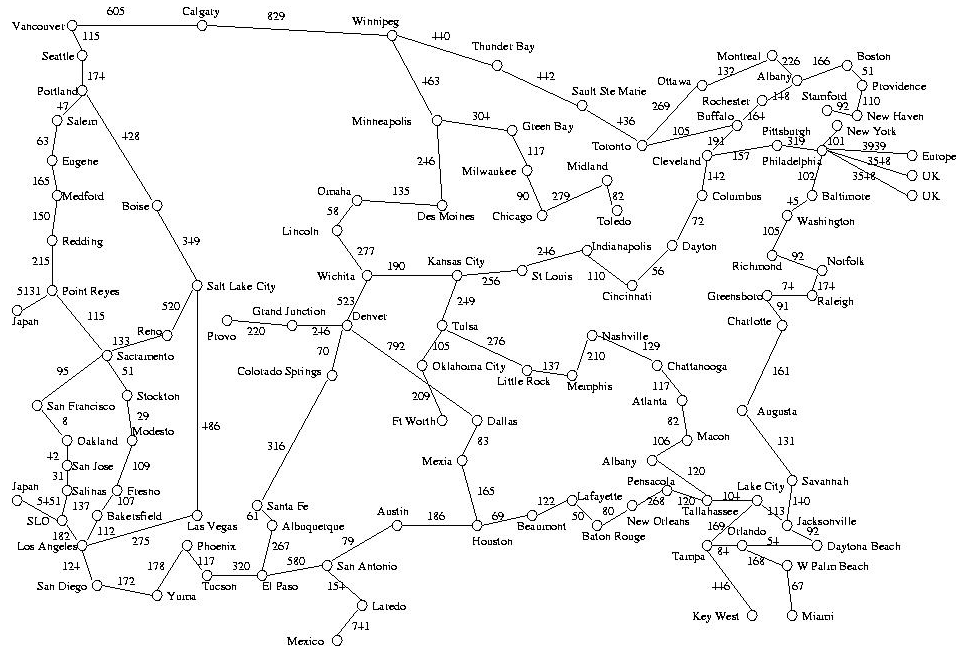
\includegraphics[scale=0.35]{map.png}
	\end{center}
	\end{figure} 
The road system is implemented as Prolog procedures in usroads.pl. \\
A node is said to be expanded when it is taken off a data structure and its successors generated. In this code, the structure is a priority queue implemented as a sorted list. (There are more efficient ways to implement such queues.) \\
The straight-line distance between cities is computed using decimal degrees of latitude and longitude by heuristic.pl. \\
Using straight-line distance as the heuristic, and starting from the astar.pl implementation, modify the code into a working Prolog implementation of A*, then perform some experiments. \\
The following modifications to the code will be necessary before you start: 
	\begin{enumerate}
  		\item The map indicates distances in miles, while the heuristic code uses kilometers as the units. Change the heuristic code to use miles.
  		\item The heuristic uses 45 degrees North latitude for all node pairs, which doesn't work well in North America. Change the heuristic code to use the average latitude of the two cities instead of 45 degrees.
  		\item Name this new heuristic source file heuristic2.pl. For ease of use, you can keep the procedure name heuristic/3.
	\end{enumerate}
	\textbf{The subproblems: }\\
	\begin{enumerate}
  		\item Submit your modified code for the heuristic. 
		\item Submit your modified code for branch-and-bound, greedy, and dynamic programming As part of your answer, compare the solution paths and explain what happened, especially any weird behavior you might detect. 
	\end{enumerate}
	
	
	\item (35 pts.) Consider the game-tree in the figure below. The leaf node contain the values generated by some unknown static evaluation function. The root node (level 0) represents the current state of the game and agent must pick the next best state to move to.
	%\usepackage{graphics} is needed for \includegraphics
\begin{figure}[h]
\begin{center}
  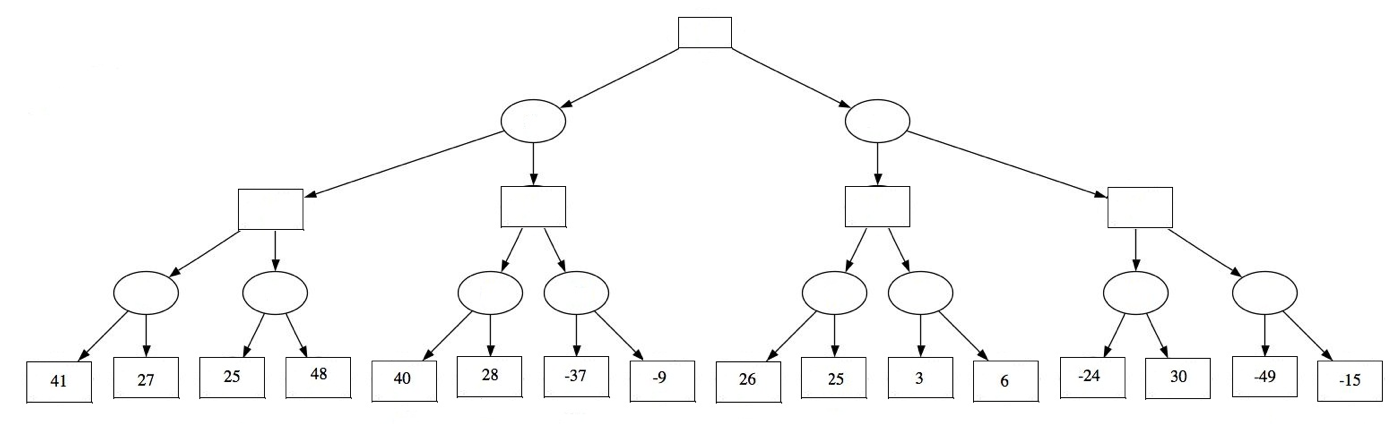
\includegraphics[scale=0.3]{tree.png}
\end{center}
\end{figure}

Now, answer the following questions: \\
	\begin{enumerate}
  		\item (8 pts.) Explore the game-tree just as the agent would using Min-Max algorithm discussed in class. At each level i, indicate the value of the nodes. Indicate the next best state picked by the agent.
  		\item (12 pts.) Explore the game-tree just as the agent would using Alpha-beta pruning discussed in class. At each level i, indicate the value of the nodes and indicate the correct set of nodes that will be pruned. You do not have to label alpha and beta. Indicate the next best state picked by the agent.
  		\item (5 pts.) What is the worst case for alpha-beta pruning? In the worst case, is the performance of alpha-beta pruning the same as min-max?
  		\item (10 pts.) Assuming that the values in the leaf nodes, the depth and branching factor remain the same, rearrange the leaves so that the new configuration represents the worst case behavior for alpha-beta pruning. Show the resulting graph and repeat 2b.
	\end{enumerate}

	\item (20 pts.) Ex. 10.4, p. 397 in the textbook.  
\end{enumerate}
\end{document}
